\section{Аналитические раздел}

\subsection{Методы получения последовательности случайных чисел}

Существует три метода получения последовательности случайных чисел:

\begin{enumerate}
	\item аппаратный (физический);
	\item табличный (файловый);
	\item алгоритмический (программный).
\end{enumerate}

\subsection{Табличная схема}

Случайные числа оформляются в виде таблицы и помещаются во внешнюю или оперативную память

\subsection{Алгоритмический способ}

Способ основан на формировании случайных чисел с помощью
специальных алгоритмов. Очередное полученное значение используется для
генерации последующих чисел.

В данной работе был использован мультипликативным конгруэнтный
метод. Последовательность вычисляется по формуле:

\begin{equation}
	X_{n+1} = (aX_{n} + c) \mod m, n \geqslant 1, при c = 0.
\end{equation}

Самым известным генератором подобного рода является так называемый
минимальный стандартный генератор случайных чисел, предложенный
Стивеном Парком и Кейтом Миллером в 1988 году. Для него a = 16807,
m = 2147483647.

В данной лабораторной работе в качестве начального значения $X_{1}$
используется текущее время в секундах.

\subsection{Критерий оценки}

В качестве критерии оценки случайности последовательности взят
критерий знаково-рейтинговый критерий Холлина, основанный на статистике:

\begin{equation}
	r = \frac{1}{k(n-1)}\sum^{n}_{i=2} \delta ((x_i - \overset{\thicksim}{x})(x_i \cdot \overset{\thicksim}{x})) R_i R_{i-1},
\end{equation}

где

\begin{enumerate}
	\item k --- коэффициент, зависящий от объема выборки (значения подбираются
	по таблице);
	\item $\overset{\thicksim}{x}$ --- медиана вариационного ряда $x_{(1)} \leqslant x_{(2)} \leqslant \dots \leqslant x_{(n)}$;
	\item $R_i$ --- ранг величины $z_i = |x_i - \overset{\thicksim}{x}| $  упорядоченном по возрастанию
	ряду значений $z_{1} \leqslant z_{2} \leqslant \dots \leqslant z_{n}$;
	\item $\delta = 
	\begin{cases}
		1,& y > 0 \\
		-1 & y < 0 \\
		0,& y = 0 \\
	\end{cases}
	$
\end{enumerate}

Ряд значений $x_i$ признается случайным, если $|r| < r_a$ 

\section{Результаты работы}

На рисунке \ref{fig:r2} представлен результат работы программы cо случайными числами.

\begin{figure}[ht!]
	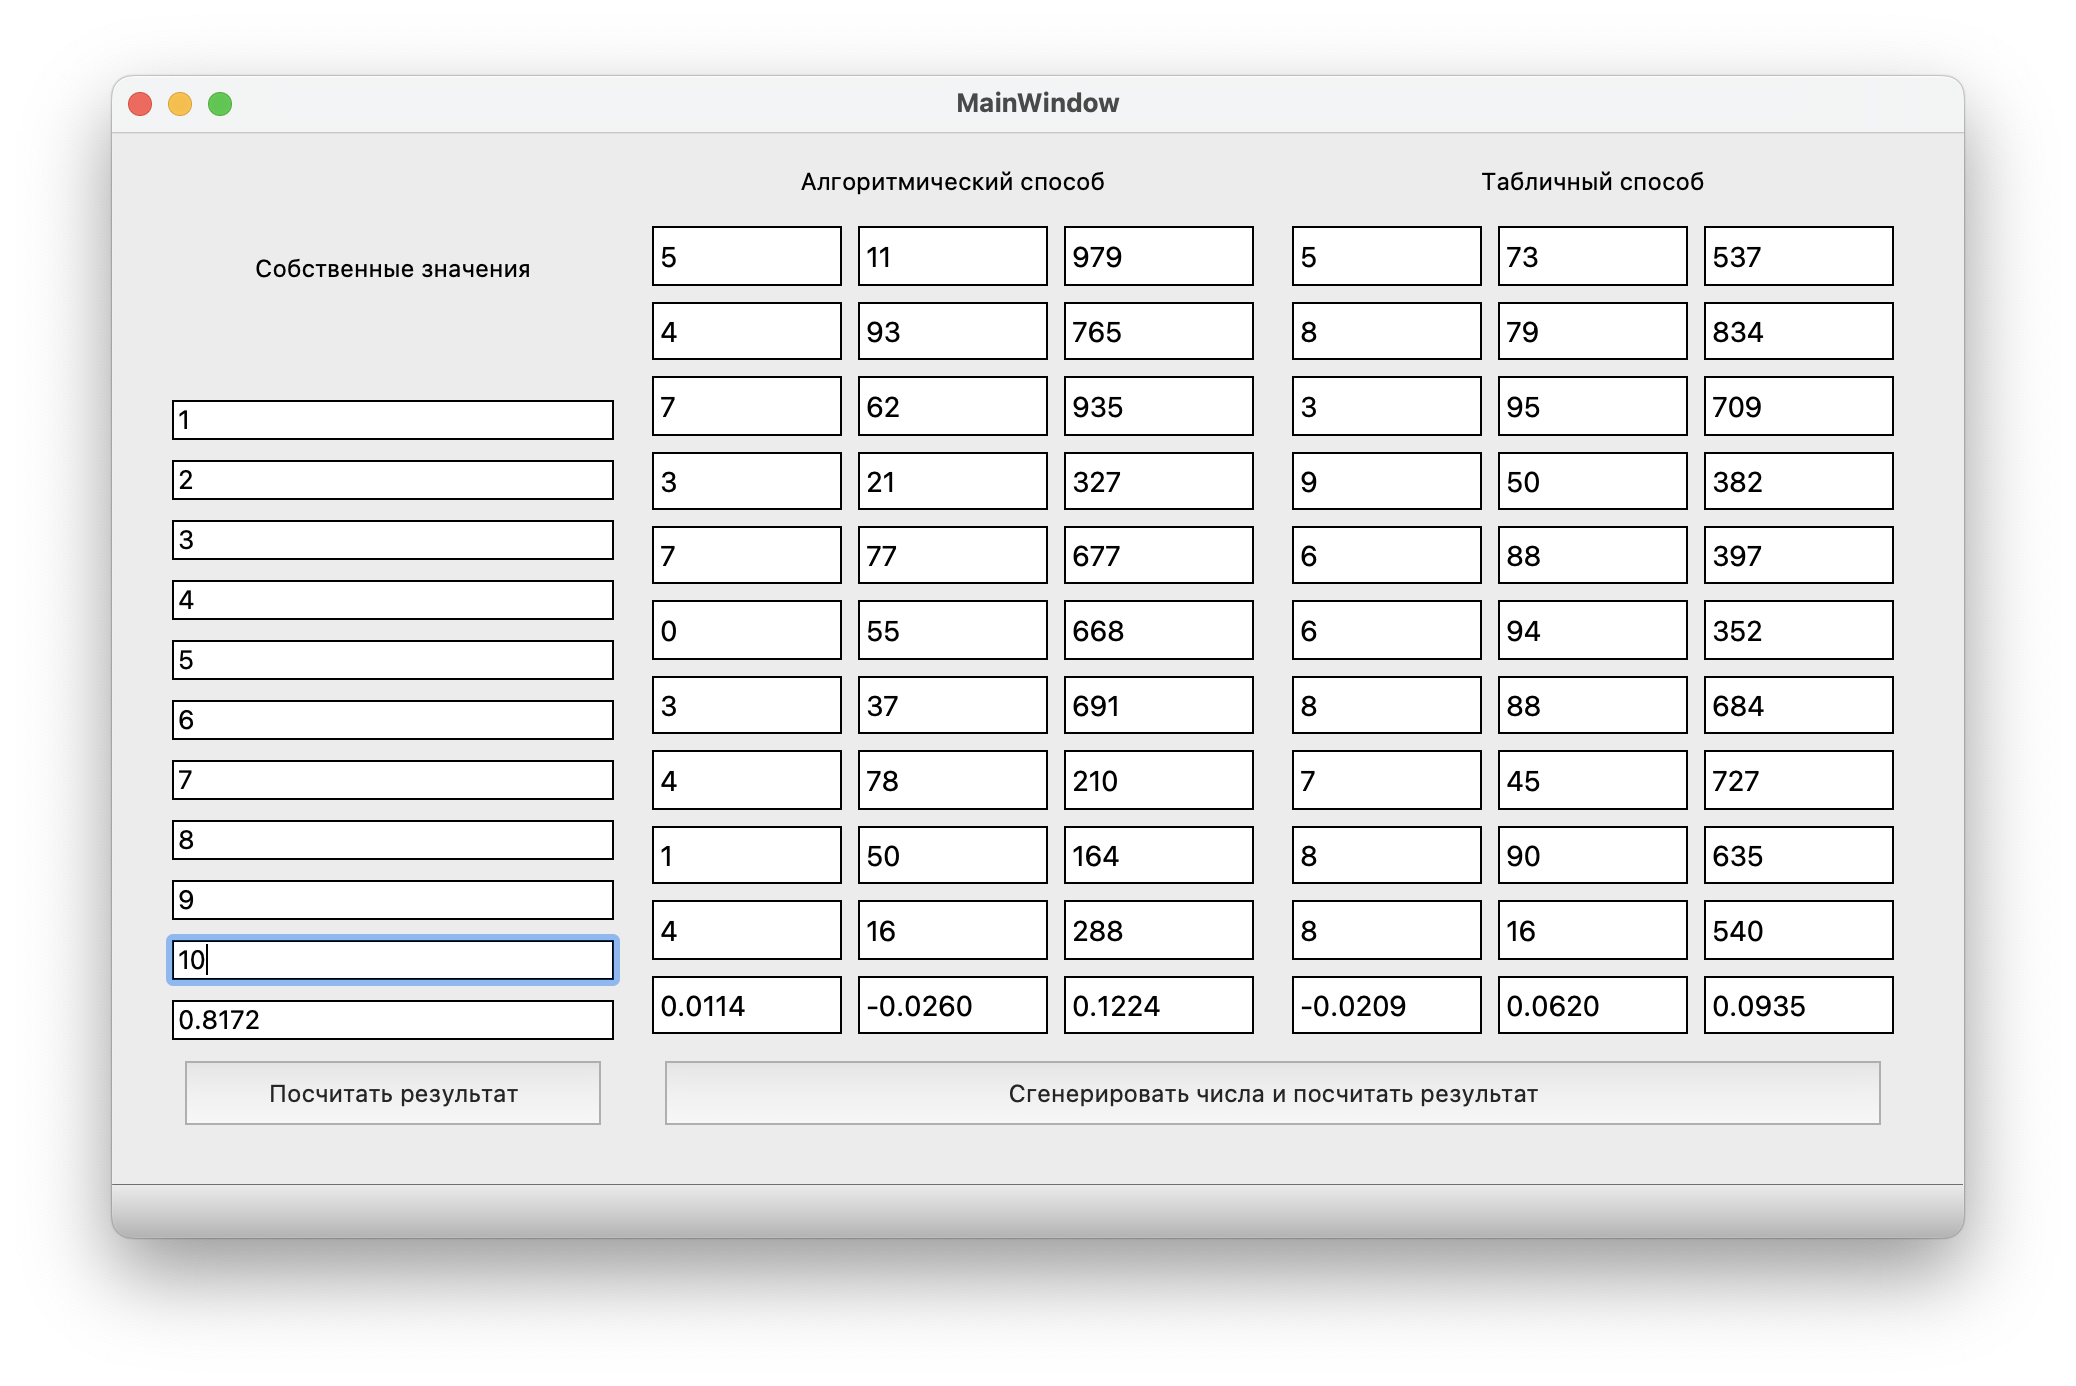
\includegraphics[width=0.75\linewidth]{assets/images/res.png}
	\caption{Результат работы программы cо случайными числами}
	\label{fig:r2}
\end{figure}